\section{The Quantum ALU's circuit}

We will implement the Quantum ALU as any other Quantum circuit we have already presented. This Quantum circuit will have
in total sixteen qubits. The first two-qubit Quantum register is called the \textit{opcode} register and it stores the bitstring
of which operation the Quantum ALU must complete, the two two-qubit general purpose Quantum registers $A$ and $B$ is where
we store the binary encoded numbers we want to be operating, the eig!ht-qubit output Quantum register $Out$ where it is used to
store the output of each operation and lastly, the two-qubit status Quantum register $Status$ where each qubit corresponds to
a logic flag.

\begin{figure}[!ht]
    \centering
    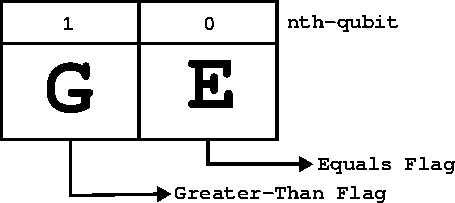
\includegraphics[scale=0.8]{images/6_Complete_System/status_reg_diagram.pdf}
    \caption{The diagram of the Status Quantum registers}
\end{figure}

\begin{listing}[!ht]
    \centering
    \begin{minted}{python3}
        from qiskit import QuantumCircuit, QuantumRegister

        op = QuantumRegister(2, name="Opcode")
        a = QuantumRegister(2, name="A")
        b = QuantumRegister(2, name="B")
        out = QuantumRegister(8, name="Out")
        stat = QuantumRegister(2, name="Status")

        qalu = QuantumCircuit(op, a, b, out, stat)
    \end{minted}
    \caption{The initialization Python code for the Quantum circuit of the Quantum ALU}
\end{listing}

After the initialization of the circuit we have to append each of the Quantum circuits that implement each of the operations
as custom Quantum gates.

To control when each of the operation will be selected accordingly to the opcode bitstring we are going to use the member
method \verb|control()| of the \verb|Gate| class. This function takes numerous parameters but we are going to use only
two of those: the \verb|num_control_qubits| and the \verb|ctrl_state| parameters. The \verb|num_control_qubits| stores
how many qubits will be used control qubits to signal the activation of the gate and the \verb|ctrl_state| parameter
annotates what is the control state of each of the control qubits. For instance, the bitstring \verb|"101"| annotates
that the least-significant and most-significant qubits will be true when in the $\ket{1}$ state and the qubit in position
1 is going to be true in the $\ket{0}$ state (inverse logic).

Using this method it is very easy to map each gate/operation to the appropriate opcode bitstring: \\\verb|ctrl_state="10"| for
the multiplication gate and \verb|ctrl_state="11"| for the comparison gate. We just have to supply the opcode register
when appending.

The addition and subtraction operations where left last because they are not that straig!ht-forward to append. These operations are
implemented by one gate that can change its mode by a control signal as an independent input. The other two operations needed
to set the \verb|num_ctrl_qubits=2| because they did not use a control signal as an input. This means that we can use one qubit
of the opcode register as an input for the Quantum Adder-Subtractor and thus we have to set \verb|num_ctrl_qubits=2| and
\verb|ctrl_state="0"| because according to the opcode table the most-significant qubit of the those operations is always in the
$\ket{0}$ state.

\begin{listing}[!ht]
    \begin{minted}{python3}
        qalu.append(addsub.control(1, ctrl_state="0"),\
            ([op[1]] + [op[0]] + a[:] + b[:] + out[:n+1]))
        qalu.append(mul.control(2, ctrl_state="10"),\
            (op[:] + a[:] + b[:] + out[:]))
        qalu.append(cmp.control(2, ctrl_state="11"),\
            (op[:] + a[:] + b[:] + out[:n+1] + stat[:]))
    \end{minted}
    \caption{Appending the custom Quantum gates of the operations to the Quantum ALU}
\end{listing}

\begin{figure}[!ht]
    \centering
    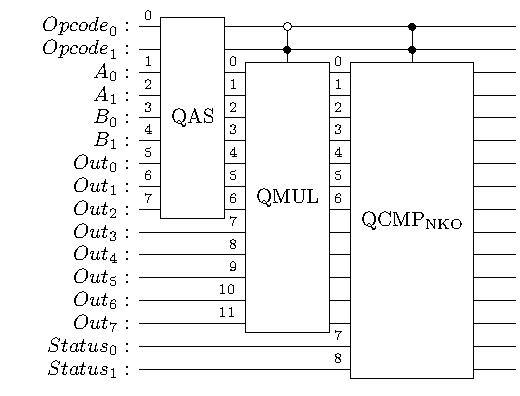
\includegraphics{images/6_Complete_System/qalu_complete.pdf}
    \caption{The Quantum circuit diagram of the Quantum ALU}
\end{figure}